\chapter*{Dodatak: Prikaz aktivnosti grupe}
		\addcontentsline{toc}{chapter}{Dodatak: Prikaz aktivnosti grupe}
		
		\section*{Dnevnik sastajanja}
		
		\begin{packed_enum}
			\item  sastanak
			
			\item[] \begin{packed_item}
				\item Datum: \date[{19. listopada 2023.}
				\item Prisustvovali: D. Matić, L. Crvelin, V. Kumanović, M. Lešković, K. Valečić, M. Vidaković
				\item Trajanje: 35min
				\item Teme sastanka:
				\begin{packed_item}
					\item  izbor tehnologije
					\item  izbor teme
                    \item  ime tima
                    \item  osnovna podjela posla
                    \item  osiguravanje pristupa na sve servisa svim članovima tima
				\end{packed_item}
            \item Zaključak: \\Dogovoreni su taskovi za prvi sprint (do četvrtrka 26.10). Oni za većinu ljudi uključuju učenje gita i tehnologija koje su odabrali (backend/frontend), a L. Crvelin treba i napraviti prve korake u organizaciji dokumentacije. Voditelj D. Matić će postaviti repozitorij na GitHubu i osigurati svima pristup. Dogovorena je i radionica na temu značajki (featurea) aplikacije sutra u 12 sati, gdje ćemo pokušati prioritizirati posao i složiti Jiru.
			\end{packed_item}

   
			\item  sastanak
			\item[] \begin{packed_item}
				\item Datum: \date[{20. listopada 2023.}
				\item Prisustvovali:  D. Matić, L. Crvelin, V. Kumanović, M. Lešković, K. Valečić, M. Vidaković
				\item Trajanje: 1h 45min
				\item Teme sastanka:
				\begin{packed_item}
					\item  analiziranje značajki aplikacije i napisati iz njih epice i storije u Jiri
					\item  stvaranje dijagrama
                    \item  daljnja podjela posla
				\end{packed_item}
            \item Zaključak: \\Detaljno su analizirane značajke aplikacije i stvoreni dijagrami iz kojih se može stvoriti definicija baze podataka što će do kraja sprinta učiniti V. Kumanović i prioritizirani popis zadataka koji će u Jiri stvoriti D. Matić. Također, identificirali smo nejasnoće u samoj definiciji zadatka koje ćemo prenijeti asistentici.
            M. Vidaković će do kraja sprinta istražiti kako se pravilno postavlja Spring projekt, a K. Valečić će isto učiniti za React u čemu će mu pomoći M. Lešković. \\
            Dogovorene su još dvije radionice sljedeći tjedan, u četvrtak i petak na temu postavljanja Reacta i Springa.
			\end{packed_item}


            \item  sastanak
			\item[] \begin{packed_item}
				\item Datum: \date[{26. listopada 2023.}
				\item Prisustvovali: D. Matić, L. Crvelin, L. Cvetkovski, V. Kumanović, M. Lešković, K. Valečić, M. Vidaković 
				\item Trajanje: 1h 30min
				\item Teme sastanka:
				\begin{packed_item}
					\item  planiranje i praćenje napretka
					\item  postavljanje backend-a prema svim pravilima i omogućavanje nesmetanog razvoja u budućnosti.
				\end{packed_item}
            \item Zaključak: \\
            Potvrdili smo da svi imaju potreban pristup na JIRU i GitHub repozitoriju. \\
             L. Crvelin je izložila napredak u dokumentiranju i predstavila način prikupljanja podataka za pojedine dijelove dokumentacije. Podaci o napretku će se prikupljati kroz komentare na JIRA taskovima i kroz bilješke sa sastanaka. Sljedeći koraci vezani uz izradu dokumentacije su raspisivanje obrazaca uporabe i pisanje opisa projektnog zadatka. To će preuzeti L. Crvelin i V. Kumanović. Također, L. Crvelin je naglasila važnost praćenja potrošenog vremena za svaki zadatak koji radimo. To će u JIRI postaviti D. Matić. \\
             Predstavljena je i schema baze podataka koju smo komentirali i utvrdili koje su potrebne promjene. Te će promjene u ovom sprintu učiniti V. Kumanović i M. Vidaković te će ih predstaviti timu na sljedećem planiranju sprinta u četvrtak. \\
             M. Vidaković je prezentirala napredak vezan uz postavljanje Spring backenda i preuzela zadatak integracije backenda s Postgresom što se može događati usporedno uz razvijanje scheme baze. \\
             K. Valečić i M. Lešković su potvrdili da su spremni za nadolazeću radionicu vezanu uz postavljanje Reacta, koja će se održati sutra (petak, 27.10. u 14 sati). Nakon te radionice bit ćemo spremni za početak razvoja na frontendu, što će preuzeti L. Cvetkovski i K. Valečić. \\
             Komentirali smo rad s gitom te je M. Lešković pokazao workflow u GitHub Desktop alatu. Naglašena je važnost da više ljudi pogleda PR prije mergea s glavnom granom.
            
			\end{packed_item}

               \item  sastanak
			\item[] \begin{packed_item}
				\item Datum: \date[{27. listopada 2023.}
				\item Prisustvovali:  D. Matić, L. Crvelin, L. Cvetkovski, V. Kumanović, M. Lešković, K. Valečić
				\item Trajanje: 45min
				\item Teme sastanka:
				\begin{packed_item}
					\item  planiranje i praćenje napretka
					\item  postavljanje frontend-a prema svim pravilima i omogućavanje nesmetanog razvoja u budućnosti
				\end{packed_item}
            \item Zaključak: \\
            M. Lešković je postavio temelje React projekta i detaljno objasnio što i kako radi. Dogovorili smo se da ćemo za izgradnju korisničkog sučelja koristiti Bootstrap, a integraciju Bootstrapa s projektom će napraviti L. Cvetkovski. Za to vrijeme će K. Valečić naučiti kako se Bootstrap koristi i onda s L. Cvetkovski izgraditi prvih nekoliko stranica aplikacije (login/register, homepage, profile edit page) do kraja ovog sprinta. M. Lešković će od sad raditi na backend dijelu. \\
            Dogovorili smo se da ćemo dodati README na projekt s uputama kako pokrenuti backend / frontend. To je bitno da svi mogu jednostavno postaviti projekt na svojim računalima.
			\end{packed_item}

            \item  sastanak
			\item[] \begin{packed_item}
				\item Datum: \date[{31. listopada 2023.}
				\item Prisustvovali:  D. Matić, L. Crvelin, L. Cvetkovski, V. Kumanović, M. Lešković, K. Valečić, M. Vidaković
				\item Trajanje: 45min
				\item Teme sastanka:
				\begin{packed_item}
					\item  praćenje napretka na frontendu
					\item  pregled funkcionalnih zahtjeva
				\end{packed_item}
                \item Zaključak: \\
                L. Crvelin je pokazala dosadašnji napredak vezan uz definiranje funkcionalnih zahtjeva i izložila nejasnoće koje imamo u ovom trenutku. Kroz raspravu smo razjasnili sve i omogućili daljnji razvoj dokumentacije.
                L. Cvetkovski je pokazao napredak vezan uz razvoj frontenda. Dogovoreno je da će frontend tim imati zasebne sastanke u terminu u kojem se dogovore kako bi odredili sljedeće korake.
            
			\end{packed_item}

            \item  sastanak
			\item[] \begin{packed_item}
				\item Datum: \date[{1. studenoga 2023.}
				\item Prisustvovali: L. Crvelin, L. Cvetkovski, M. Lešković
				\item Trajanje: 1h
				\item Teme sastanka:
				\begin{packed_item}
					\item  Razdvajanje uloga
                    \item Određivanje podstranica za svaku ulogu
                    \item Pregled dosadašnjeg napretka
                    \item podjela zadatka
				\end{packed_item}
                \item Zaključak: \\
                Dogovoreno je da trebamo razdvojiti uloge na platformi, odnosno definirati različite korisničke uloge: pedijatar, liječnik obiteljske medicine (OM), i roditelj.
                Razgovarali smo o potrebi definiranja specifičnih podstranica za svaku ulogu kako bismo omogućili prilagođeni sadržaj i funkcionalnosti za svaku kategoriju korisnika.
                Odlučeno je da će adminu biti omogućeno upravljanje svim računima korisnika s jedne centralne stranice nazvane "racuni.js". Ovo će pojednostaviti administraciju i omogućiti efikasnije upravljanje korisničkim računima.
                Razgovarali smo o raspodjeli zadatka za izradu osnovnih kostura stranica za svaku ulogu na frontendu. L. Cvetkovski će raditi na stranici za pedijatra i liječnika obiteljske medicine, a K. Valečić će raditi na stranici za roditelja.
			\end{packed_item}

            \item  sastanak
			\item[] \begin{packed_item}
				\item Datum: \date[{1. studenoga 2023.}
				\item Prisustvovali: D. Matić, M. Vidaković
				\item Trajanje: 45min
				\item Teme sastanka: 
				\begin{packed_item}
					\item  projektiranje baze podataka
				\end{packed_item}
                \item Zaključak: \\
                
			\end{packed_item}
			

            \item  sastanak
			\item[] \begin{packed_item}
				\item Datum: \date[{2. studenoga 2023.}
				\item Prisustvovali: D. Matić, L. Crvelin, L. Cvetkovski, V. Kumanović, M. Lešković, K. Valečić, M. Vidaković
				\item Trajanje: 2h 45min
				\item Teme sastanka: 
				\begin{packed_item}
					\item  planiranje i praćenje napretka
				\end{packed_item}
                \item Zaključak: \\
                Dogovorili smo sljedeće korake koje treba napraviti vezano uz dokumentaciju kako bismo mogli tražiti povratnu
                informaciju na konzulatcijama u utorak (7.11). L. Crvelin će prepisati definirane tablice baze iz Excela u
                dokumentaciju, a V. Kumanović će iz definiranih tablica nacrtati dijagram baze podataka koji je također dio
                dokumentacije. Prošli smo kroz sve obrasce uporabe koje smo do sad definirali i dogovorili se da će oni biti dovršeni do
                ponedjeljka, što će učiniti L. Crvelin. \\
                
                D. Matić je pokazao napredak u izboru i postavljanju deploy platforme. Izabrali smo Heroku i napravili osnovno
                postavljenje dviju aplikacija (frontend i backend). \\
                
                M. Vidaković je pokazala kako se Postgres baza spaja na Spring aplikaciju što nam je bio preduvjet da možemo nastaviti
                razvoj na backendu, ali i da možemo napraviti potpun deployment aplikacije. Nastavno na to će M. Lešković
                implementirati mehanizme za prijavu i registraciju korisnika pomoću Spring Security modula, a D. Matić će napraviti
                potrebne korake na Heroku platformi vezane uz deploy aplikacije. M. Vidaković će u sljedećem sprintu implementirati
                mehanizam uloga na entitetu korisnika. \\
                
                L. Cvetkovski i K. Valečić su podijelili plan za razvoj frontenda s ostalima. Potvrdili smo daljnje korake
                vezane uz razvoj React aplikacije koji uključuju restrukturiranje i razvoj homescreena. Dogovoreno je da će frontend tim
                razraditi najbolje načine kako nastaviti raditi s obzirom da backend još uvijek zaostaje za frontendom.
               
			\end{packed_item}

			\item  sastanak
			\item[] \begin{packed_item}
				\item Datum: \date[{9. studenoga 2023.}
				\item Prisustvovali: D. Matić, L. Crvelin, L. Cvetkovski, V. Kumanović, M. Lešković, K. Valečić, M. Vidaković
				\item Trajanje: 1h 30min
				\item Teme sastanka: 
				\begin{packed_item}
					\item  planiranje i praćenje napretka
				\end{packed_item}
                \item Zaključak: \\
				Analizirali smo povratne informacije koje smo dobili na konzultacijama u utorak i podijelili posao vezan uz to 
				u ovom sprintu. L. Crvelin će napraviti sve potrebne promjene na UC-ovima,  Vedran Kumanović će modificirati dijagram 
				baze podataka, a Dorian Matić će dovršiti odlomak "Arhitektura sustava". \\
 
				Leon Cvetkovski je predstavio napredak u refaktoriziranju frontenda koji su on i Krešimir Valečić napravili u ovom sprintu.
				Zaključili smo da je frontend sad spreman za spajanje s backendom. \\
				 
				Mihael Lešković je opisao probleme s kojima se susreo pri postavljanju Spring Security modula za backend aplikacije. 
				Dogovoreno je da će on i Dorian Matić probati što prije to popraviti i omogućiti daljnju razvoj frontenda.
               
			\end{packed_item}

			\item  sastanak
			\item[] \begin{packed_item}
				\item Datum: \date[{11. studenoga 2023.}
				\item Prisustvovali: D. Matić, L. Cvetkovski, M. Lešković, K. Valečić
				\item Trajanje: 1h 30min
				\item Teme sastanka: 
				\begin{packed_item}
					\item  Omogućiti frontend timu da spoji React aplikaciju s backendom
				\end{packed_item}
                \item Zaključak: \\
                Predstavljen je dio backenda vezan uz Spring Security. Frontend tim je naučio kako se pokreće backend aplikacija lokalno.
                Dogovoreni su sljedeći koraci.
				
               
			\end{packed_item}

			\item  sastanak
			\item[] \begin{packed_item}
				\item Datum: \date[{16. studenoga 2023.}
				\item Prisustvovali: D. Matić, L. Crvelin, L. Cvetkovski, V. Kumanović, M. Lešković, K. Valečić, M. Vidaković
				\item Trajanje: 45min
				\item Teme sastanka: 
				\begin{packed_item}
					\item  planiranje i praćenje napretka
				\end{packed_item}
                \item Zaključak: \\
                Timovi za dokumentaciju, backend i frontend su predstavili svoj napredak u ovom sprintu. Dogovorene su zadnje promjene
				u dokumentaciji prije verzije 1.0.\\
				Dogovoreno je da sljedeći sprint zbog međuispita kreće tek u četvrtak, 30.11. Do tad, svi timovi trebaju smisliti
				prijedloge daljenjeg djelovanja. Svi članovi tima su pristali na cilj da cjelokupna funkcionalnost aplikacije bude
				gotova do 1.1.2024.
                
               
			\end{packed_item}

			\item  sastanak
			\item[] \begin{packed_item}
				\item Datum: \date[{30. studenoga 2023.}
				\item Prisustvovali: D. Matić, L. Cvetkovski, V. Kumanović, M. Lešković, K. Valečić, M. Vidaković
				\item Trajanje: 40min
				\item Teme sastanka: 
				\begin{packed_item}
					\item  planiranje i praćenje napretka
				\end{packed_item}
                \item Zaključak: \\
                Dogovoreni su daljni koraci za frontend, backend i dokumentaciju. Vedran Kumanović će istražiti koji su nam 
				dijagrami potrebni u dokumentaciji i koji podaci nam trebaju kako bismo ih izradili. Analizirat će kako te 
				podatke prikupiti i imamo li ih već prikupljene. Osim toga, napisat će i odlomak "Upute za puštanje u rad aplikacije"
				 u dokumentaciji, na temelju README-ja. \\
 				Mihael Lešković će nastaviti razvijati podršku za usere tako što će implementirati sve atribute usera unutar 
				aplikacije i također njihove validacije. Mia Vidaković će nastaviti raditi na implementaciji uloga unutar aplikacije.\\
 				Krešimir Valečić i Leon Cvetkovski će nadograditi ekran za registraciju s novim poljima koja su potrebna i napravit 
				će novi ekran za unos ili izmjenu atributa usera.
			
			\end{packed_item}

			\item  sastanak
			\item[] \begin{packed_item}
				\item Datum: \date[{4. prosinca 2023.}
				\item Prisustvovali: D. Matić, M. Lešković, K. Valečić, M. Vidaković
				\item Trajanje: 40min
				\item Teme sastanka: 
				\begin{packed_item}
					\item  
				\end{packed_item}
                \item Zaključak: \\
                
			
			\end{packed_item}

			\item  sastanak
			\item[] \begin{packed_item}
				\item Datum: \date[{7. prosinca 2023.}
				\item Prisustvovali: D. Matić, L. Crvelin, V. Kumanović, M. Lešković, K. Valečić, M. Vidaković
				\item Trajanje: 1h 5min
				\item Teme sastanka: 
				\begin{packed_item}
					\item  planiranje i praćenje napretka
				\end{packed_item}
                \item Zaključak: \\
                Dogovoreno je da će se tijekom sljedećeg sprinta napraviti radionica vezana uz preostale dijagrame koje treba nacrtati
tim za dokumentaciju će predstaviti kakvi su to dijagrami i prikupiti informacije potrebne da ih se nacrta.\\

Vedran Kumanović mora završtiti odlomak "Upute za puštanje u rad aplikacije", što mu je ostalo od prethodnog sprinta.\\

Leon Cvetkovski i Krešimir Valečić moraju završiti ekrane koji su im ostali od prošlog sprinta i nastaviti raditi na
ekranima za preglede i spajanje doktora i pacijenata.\\

Mia Vidaković će nastaviti s implementacijama uloga, a Mihael Lešković će nastaviti rad na korisnicima i pregledima.
                
			
			\end{packed_item}

			\item  sastanak
			\item[] \begin{packed_item}
				\item Datum: \date[{11. prosinca 2023.}
				\item Prisustvovali: D. Matić, L. Crvelin, V. Kumanović, M. Lešković, K. Valečić, M. Vidaković
				\item Trajanje: 1 h 30 min
				\item Teme sastanka: 
				\begin{packed_item}
					\item koordinacija o napretku unutar jednog sprinta
				\end{packed_item}
                \item Zaključak: \\
                Diskusija i rješavanje tehničkh problema vezanih uz dodjeljene zadatke na frontendu i backendu.
			
			\end{packed_item}

			\item  sastanak
			\item[] \begin{packed_item}
				\item Datum: \date[{14. prosinca 2023.}
				\item Prisustvovali: D. Matić, L. Crvelin, L.Cvetkovski, V. Kumanović, M. Lešković, K. Valečić, M. Vidaković
				\item Trajanje: 1 h 30 min
				\item Teme sastanka: 
				\begin{packed_item}
					\item  planiranje i praćenje napretka
				\end{packed_item}
                \item Zaključak: \\
                Tim za dokumentaciju će pripremiti radionicu vezanu uz dijagrame stanja i komponenti, a Lucia Crvelin će napisati i
odlomak "Korištene tehnologije i alati".

Dorian Matić će provesti reviziju dokumentacije kako bismo utvrdili u koji dijelovi dokumentacije se razlikuju od
implementacije.

Frontend tim će integrirati ekrane vezane u korisnike s backendom.

Backend tim će nastaviti rad na novim entitetima i otvarati API endpointe koji su definirani u specifikaciji API-ja.
                
			
			\end{packed_item}

			\item  sastanak
			\item[] \begin{packed_item}
				\item Datum: \date[{18. prosinca 2023.}
				\item Prisustvovali: D. Matić, L. Crvelin, V. Kumanović, M. Lešković, K. Valečić, M. Vidaković
				\item Trajanje: 30min
				\item Teme sastanka: 
				\begin{packed_item}
					\item  mid-sprint sync
				\end{packed_item}
                \item Zaključak: \\
                Diskusija i rješavanje tehničkh problema vezanih uz dodjeljene zadatke na frontendu i backendu.
                
			
			\end{packed_item}

			\item  sastanak
			\item[] \begin{packed_item}
				\item Datum: \date[{21. prosinca 2023.}
				\item Prisustvovali: D. Matić, L. Crvelin, M. Lešković, V. Kumanović, K. Valečić, M. Vidaković
				\item Trajanje: 1h 30min
				\item Teme sastanka: 
				\begin{packed_item}
					\item  planiranje i praćenje napretka
				\end{packed_item}
			
			\end{packed_item}

			\item  sastanak
			\item[] \begin{packed_item}
				\item Datum: \date[{26. prosinca 2023.}
				\item Prisustvovali:  D. Matić, L. Crvelin, V. Kumanović, M. Lešković, K. Valečić, M. Vidaković
				\item Trajanje: 1 h 30 min
				\item Teme sastanka: 
				\begin{packed_item}
					\item koordinacija o napretku unutar jednog sprinta
				\end{packed_item}
                \item Zaključak: \\
                Diskusija i rješavanje tehničkh problema vezanih uz dodjeljene zadatke na frontendu i backendu.
			
			\end{packed_item}

			\item  sastanak
			\item[] \begin{packed_item}
				\item Datum: \date[{28. prosinca 2023.}
				\item Prisustvovali: D. Matić, L. Crvelin, M. Lešković, M. Vidaković
				\item Trajanje: 1h
				\item Teme sastanka: 
				\begin{packed_item}
					\item  planiranje i praćenje napretka
				\end{packed_item}
                \item Zaključak: \\
                Tim za dokumentaciju će pripremiti radionicu vezanu uz dijagrame stanja i komponenti, a Lucia Crvelin će napisati i
odlomak "Korištene tehnologije i alati".

Dorian Matić će provesti reviziju dokumentacije kako bismo utvrdili u koji dijelovi dokumentacije se razlikuju od
implementacije.

Frontend tim će integrirati ekrane vezane u korisnike s backendom.

Backend tim će nastaviti rad na novim entitetima i otvarati API endpointe koji su definirani u specifikaciji API-ja.
                
			
			\end{packed_item}

			\item  sastanak
			\item[] \begin{packed_item}
				\item Datum: \date[{2. siječnja 2024.}
				\item Prisustvovali: D. Matić, L. Crvelin, M. Lešković
				\item Trajanje: 30 min
				\item Teme sastanka: 
				\begin{packed_item}
					\item  mid-sprint sync
				\end{packed_item}
                \item Zaključak: \\
                Diskusija i rješavanje tehničkh problema vezanih uz dodjeljene zadatke na frontendu i backendu.
                
			
			\end{packed_item}

			\item  sastanak
			\item[] \begin{packed_item}
				\item Datum: \date[{4. siječnja 2024.}
				\item Prisustvovali: D. Matić, L. Crvelin, L. Cvetkovski, M. Lešković, M. Vidaković
				\item Trajanje: 1 h
				\item Teme sastanka: 
				\begin{packed_item}
					\item  planiranje i praćenje napretka
				\end{packed_item}
              
			\end{packed_item}

			\item  sastanak
			\item[] \begin{packed_item}
				\item Datum: \date[{11. siječnja 2024.}
				\item Prisustvovali:  D. Matić, L. Crvelin, L. Cvetkovski, V. Kumanović, M. Lešković, K. Valečić, M. Vidaković
				\item Trajanje: 1 h 30 min
				\item Teme sastanka: 
				\begin{packed_item}
					\item  planiranje i praćenje napretka
				\end{packed_item}
               
                
			\end{packed_item}

			\item  sastanak
			\item[] \begin{packed_item}
				\item Datum: \date[{15. siječnja 2024.}
				\item Prisustvovali: 
				\item Trajanje: 1h 30 min
				\item Teme sastanka:  D. Matić, L. Crvelin, M. Lešković, K. Valečić
				\begin{packed_item}
					\item  mid-sprint sync
				\end{packed_item}
                
			\end{packed_item}

			\item  sastanak
			\item[] \begin{packed_item}
				\item Datum: \date[{18. siječnja 2024.}
				\item Prisustvovali: 
				\item Trajanje: 45 min
				\item Teme sastanka: D. Matić, L. Crvelin, V. Kumanović, M. Lešković, K. Valečić, M. Vidaković
				\begin{packed_item}
					\item  planiranje i praćenje napretka
					\item verifikacija i validacija
				\end{packed_item}
                
    
			\end{packed_item}

			\item  sastanak
			\item[] \begin{packed_item}
				\item Datum: \date[{19. siječnja 2024.}
				\item Prisustvovali:  D. Matić, L. Crvelin, V. Kumanović, M. Lešković, K. Valečić, M. Vidaković
				\item Trajanje: 1 h
				\item Teme sastanka: 
				\begin{packed_item}
					\item  revizija dokumentacije
				\end{packed_item}
                
			\end{packed_item}

		\end{packed_enum}
		
		\eject
		\section*{Tablica aktivnosti}
			 %Doprinose u aktivnostima treba navesti u satima po članovima grupe po aktivnosti.}

			\begin{longtblr}[
					label=none,
				]{
					vlines,hlines,
					width = \textwidth,
					colspec={X[7, l]X[1, c]X[1, c]X[1, c]X[1, c]X[1, c]X[1, c]X[1, c]}, 
					vline{1} = {1}{text=\clap{}},
					hline{1} = {1}{text=\clap{}},
					rowhead = 1,
				} 
			
				\SetCell[c=1]{c}{} & \SetCell[c=1]{c}{\rotatebox{90}{\textbf{Dorian Matić}}} & \SetCell[c=1]{c}{\rotatebox{90}{\textbf{Lucia Crvelin }}} &	\SetCell[c=1]{c}{\rotatebox{90}{\textbf{Leon Cvetkovski }}} & \SetCell[c=1]{c}{\rotatebox{90}{\textbf{Vedran Kumanović }}} &	\SetCell[c=1]{c}{\rotatebox{90}{\textbf{Mihael Lešković }}} & \SetCell[c=1]{c}{\rotatebox{90}{\textbf{Krešimir Valečić }}} &	\SetCell[c=1]{c}{\rotatebox{90}{\textbf{Mia Vidaković }}} \\  
				Upravljanje projektom                                   & 12h  &      &     &      &      &     &     \\
				Opis projektnog zadatka                                 &      & 3.5h &     &      &      &     &     \\
				Funkcionalni zahtjevi                                   &      & 3h   &     &      &      &     &     \\
				Opis pojedinih obrazaca                                 &      & 8h   &     &      &      &     &     \\
				Dijagram obrazaca                                       &      & 5h   &     &      &      &     &     \\
				Sekvencijski dijagrami                                  &      & 4.5h &     &      &      &     &     \\
				Opis ostalih zahtjeva                                   &      & 1h   &     &      &      &     &     \\
				Arhitektura I dizajn sustava                            & 3h   &      &     &      &      &     &     \\
				Baza podataka                                           & 2h   &      &     & 5h   &      &     & 3h  \\
				Dijagram razreda                                        &      &      &     & 5h   &      &     & 1h  \\
				Dijagram stanja                                         &      &      &     & 3h   &      &     &     \\
				Dijagram aktivnosti                                     &      & 1h   &     & 2h   &      &     &     \\
				Dijagram komponenti                                     & 0.5h &      &     & 0.5h & 0.5h &     &     \\
				Korištene tehnologije I alati                           &      & 1.5h &     &      &      &     & 4h  \\
				Ispitivanje programskog rješenja                        &      &      &     &      &      & 1h  & 6h  \\
				Dijagram razmještaja                                    &      & 2h   &     &      &      &     &     \\
				Upute za puštanje u pogon                               & 1.5h &      &     & 3h   &      &     &     \\
				Dnevnik sastajanja                                      & 1h   &      &     &      &      &     &     \\
				Zaključak I budući rad                                  &      & 1.5h &     &      &      &     &     \\
				Integracija baze podataka                               &      &      &     &      &      &     & 7h  \\
				Spring security                                         & 4h   &      &     &      & 15h  &     &     \\
				Frontend inicijalizacija                                &      &      & 10  &      & 3h   & 1h  &     \\
				Deployment                                              & 6h   &      &     &      &      &     &     \\
				Backend inicijalizacija                                 &      &      &     &      &      &     & 2h  \\
				Postavljanje, revizija dokumentacije I dr.              & 2h   & 5h   &     &      &      &     &     \\
				Rad na komponentama i  ekranima (FE)                    & 2h   &      & 20h &      & 3h   & 7h  &     \\
				Rad na domenskim klasama, servisima i kontrolerima (BE) &      &      &     &      & 13h  &     & 24h \\
				Integracija FE i BE                                     & 1h   &      &     &      &      & 20h &     \\
				OpenStreetMap implementacija (FE)                       &      &      &     &      & 12h  &     &     \\
				Dopunjavanje raznih funkcionalnosti                     &      &      &     &      & 8h   &     &     \\
				Sastanci                                                & 20h  & 20h  & 20h & 20h  & 20h  & 20h & 20h  
			\end{longtblr}
					
					
		\eject
		\section*{Dijagrami pregleda promjena}
		
		%dio 2. revizije
		
		%Prenijeti dijagram pregleda promjena nad datotekama projekta. Potrebno je na kraju projekta generirane grafove s gitlaba prenijeti u ovo poglavlje dokumentacije. Dijagrami za vlastiti projekt se mogu preuzeti s gitlab.com stranice, u izborniku Repository, pritiskom na stavku Contributors.
		\begin{figure}[H]
			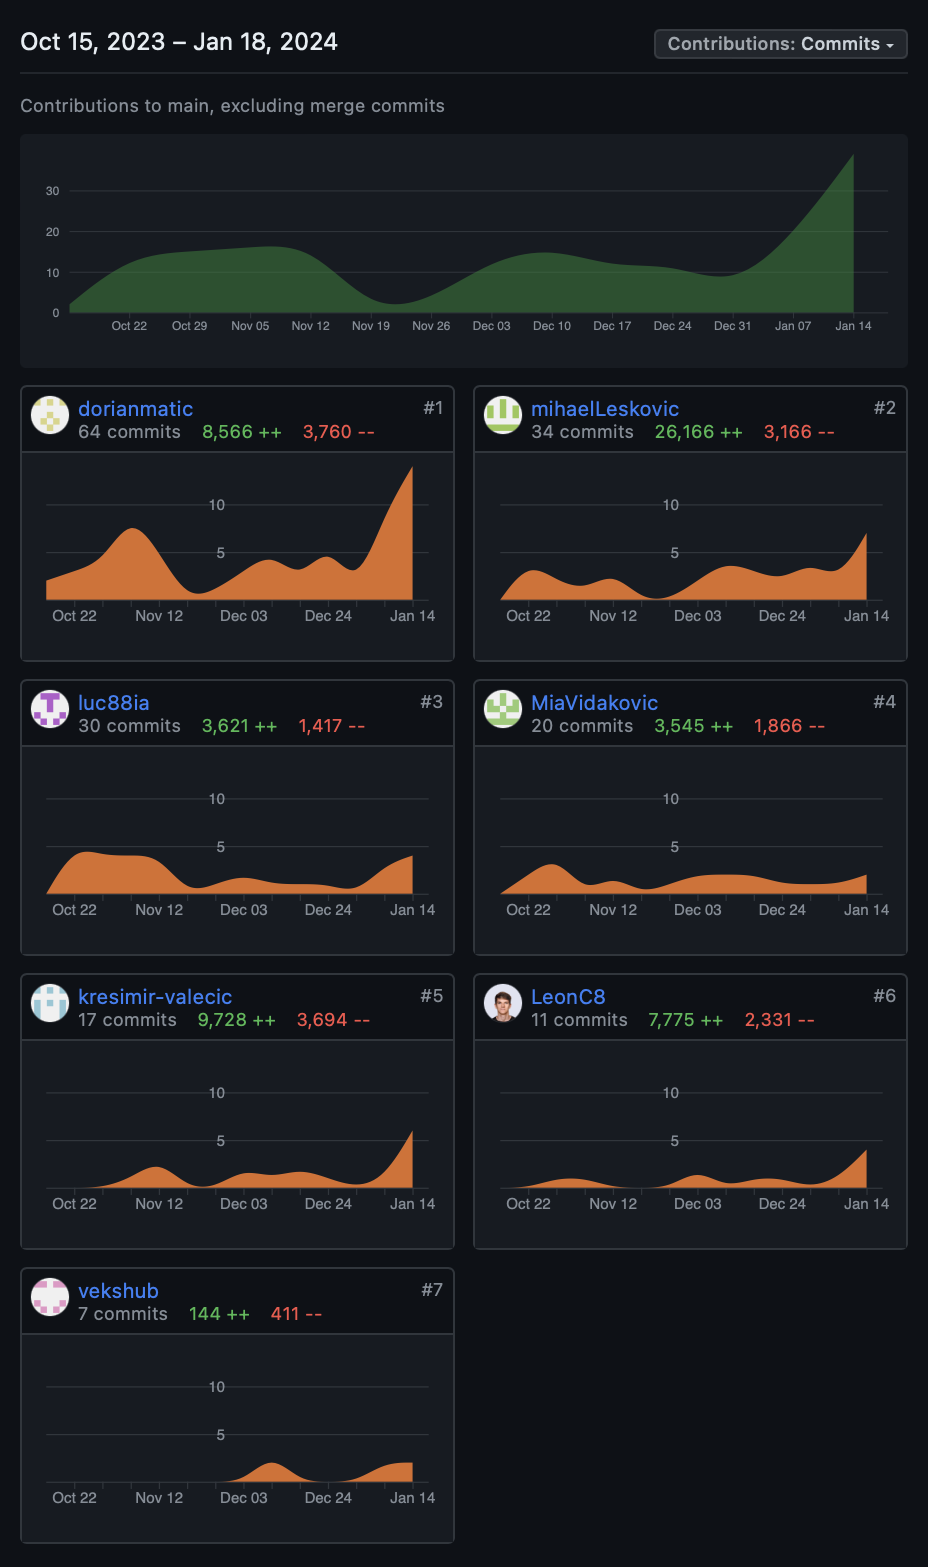
\includegraphics[width=\textwidth]{slike/pregled-promjena.png} 
			\caption{Dijagram pregleda promjena}
		\end{figure}
	